% !TEX encoding = UTF-8 Unicode

\documentclass[a4paper]{article}

\usepackage{color}
\usepackage{url}
\usepackage[T2A]{fontenc} % enable Cyrillic fonts
\usepackage[utf8]{inputenc} % make weird characters work
\usepackage{graphicx}
\usepackage{amsmath}

\usepackage[english,serbian]{babel}
%\usepackage[english,serbianc]{babel} %ukljuciti babel sa ovim opcijama, umesto gornjim, ukoliko se koristi cirilica

\usepackage[unicode]{hyperref}
\hypersetup{colorlinks,citecolor=green,filecolor=green,linkcolor=blue,urlcolor=blue}

%\newtheorem{primer}{Пример}[section] %ćirilični primer
\newtheorem{primer}{Primer}[section]

\begin{document}

\title{Etape prevođenja Haskela do mašinskog jezika\\ \small{Seminarski rad u okviru kursa\\Metodologija stručnog i naučnog rada\\ Matematički fakultet}}

\author{Marija Mijailović, Miroslav Mišljenović, Nemanja Antić, Filip Lazić\\ mijailovicmarija@hotmail.com, mr12260@alas.matf.bg.ac.rs,\\ antic.cubaka@gmail.com, filipl41@yahoo.com}
\date{april 2018.}
\maketitle

\abstract
	U ovom tekstu je ukratko prikazana osnovna forma seminarskog rada. Obratite pažnju da je pored ove .pdf datoteke, u prilogu i odgovarajuća .tex datoteka, kao i .bib datoteka korišćena za generisanje literature. Na prvoj strani seminarskog rada su naslov, apstrakt i sadržaj, i to sve mora da stane na prvu stranu! Kako bi Vaš seminarski zadovoljio standarde i očekivanja, koristite uputstva i materijale sa predavanja na temu pisanja seminarskih radova. Ovo je samo šablon koji se odnosi na fizički izgled seminarskog rada (šablon koji \emph{morate} da ispoštujete!) kao i par tehničkih pomoćnih uputstava. Molim Vas da kada budete predavali seminarski rad, imenujete datoteke tako da sadrže temu seminarskog rada, kao i imena i prezimena članova grupe (ili samo temu i prezimena, ukoliko je sa imenima predugačko). Predaja seminarskih radova biće isključivo preko web forme, a NE slanjem mejla.

%\setcounter{tocdepth}{1}
\tableofcontents

\newpage

\section{Uvod}
\label{sec:uvod}

Mnogi kompajlLeri obavljaju neki deo svog rada pomoću očuvanja ispravnosti, poboljšanja performansi, programskih transformacija. Radi konkretnosti, fokusirali smo se na Glazgov Haskel Kompajler (eng. Glasgow Haskell Compiler(GHC)) \cite{GHCxx}, ali ističemo da sve što navedemo u ovom radu se odnosi i na bilo koji kompajler funkcionalnih jezika, a možda i na kompajliranje drugih jezika. GHC preuzima ovu ideju “kompilacije transformacijom” (eng. \emph{compilation by transformation}) pokušavajući da što više izrazi proces kompilacije u obliku programskih transformacija. U ovom radu prikazaćemo u primeni transformacione tehnike kroz GHC.

\subsection{Haskel}
\label{subsec:podnaslovHaskel}
Haskel je funkcionalni jezik opšte namene, koji sadrži mnoge inovacije u dizajnu programskih jezika. Haskel podržava funkcije višeg reda (eng. \emph{ higher-order functions}), ne-striktnu semantiku, statički polimorfizam, korisnički definisane algebarske tipove, prepoznavanje šablona (eng. \emph{ pattern-matching}), rad sa listama. Razvijen je kroz sistem modula kao proširenje programskog jezika. Poseduje veliki skup primitivnih tipova uključujući liste, nizove, cele brojeve različitih namena i dužina, realne brojeve. Može se reći da je Haskel završetak dugogodišnjeg rada i istraživanja na ne-striktnim funkcionalnim jezicima \cite{Has10}. 

\subsection{GHC}
\label{subsec:podnaslovGHC}

Uobičajno se tretira kao standardna implementacija Haskela, na kojoj se baziraju i druge implementacije. Razvijan je počev od 1989. godine. GHC je pisan u Haskelu – kompajler sadrži 227,000 linija koda (uključujući komentare), a biblioteke (moduli) sadrže 242,000 linija koda (uključujući komentare). Sastavni deo svakog kompajlera za funkcionalni jezik čini i run-time sistem. Za GHC, run-time sistem je pisan u C-u i sadrži 87,000 linija koda. Tekuću verziju kompajlera, razvijalo je 23 programera (eng. developers) sa preko 500 priloga (eng. commits) \cite{StanfordGHC}.  


Celokupna struktura kompajlera se sastoji iz tri faze:
\begin{enumerate}
	\item Prva faza (eng. \emph{Frontend}) čini pretvaranje izvornog k\^{o}da pisanog u Haskelu, u takozvani Core jezik (eng. \emph {Core language}). U ovoj fazi, kompajler napisan u Haskelu, vrši analizu izvornog k\^{o}da, pravi odgovarajuće drvo izvođenja, realizuje leksičku i sintaksnu analizu, proveru tipova i kao izlaz daje k\^{o}d sa veoma redukovanim skupom instrukcija, koji zahteva Core. Više o ovoj fazi može se naći u Sekciji \ref{sec:frontend}.
	\item Druga faza (eng. \emph {Middle End}) – izlazni k\^{o}d iz prethodne faze – međujezik (eng. \emph {Intermediate language}) se dodatno optimizuje, i to kroz niz transformacija. Rezultat rada Core-a se dobija u Core obliku. Na taj način, sledeće etape transformacije k\^{o}da tačno znaju kakve konstrukcije im se mogu naći na ulazu.  Više o ovoj fazi može se naći u Sekciji \ref{sec:middle}.
	\item Treća faza (eng. \emph {Backend}) obuhvata generisanje k\^{o}da. Core-ov k\^{o}d iz prethodne faze postaje ulaz u STG-mašinu (eng. \emph {Spineless Tagless G-machine}). Rezultat rada STG-mašine se grana u tri toka. Prvi tok podrazumeva prevođenje u izvorni mašinski k\^{o}d. Drugi tok podrazumeva korišćenje LLVM-a (eng. \emph{Low-Level Virtual Machine}) za dobijanje optimizovanog k\^{o}da pomoću ove virtualne mašine. Treći tok koristi jezik C-\,- za dobijanje izvršnog k\^{o}da. Više o ovoj fazi može se naći u Sekciji \ref{sec:backend}.
\end{enumerate}

Razvojne etape pravljenja izvršnog k\^{o}da mogu se videti na slici \ref{fig:razvojneEtaple} preuzetoj sa \cite{StanfordGHC}.

\begin{figure}[h!]
	\begin{center}
		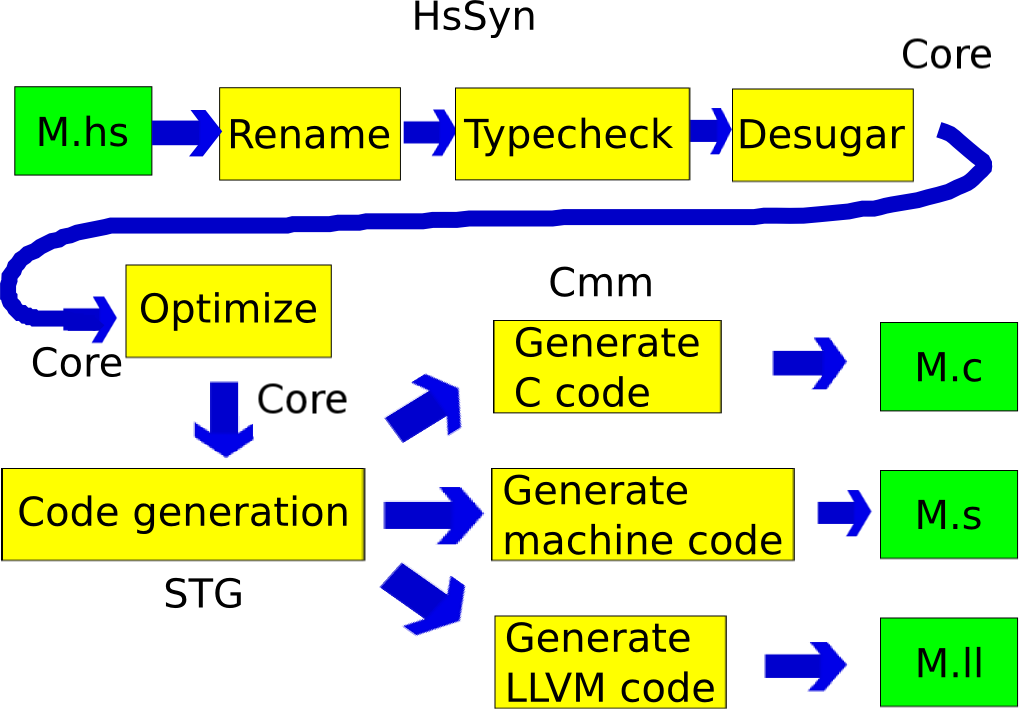
\includegraphics[scale=0.30]{resources/razvojneEtape.png}
	\end{center}
	\caption{Razvojne etape pravljenja izvršnog k\^{o}da}
	\label{fig:razvojneEtaple}
\end{figure}
\section{Front end}
\label{sec:frontend}

Kao sto smo rekli, Front end je prva faza u kojoj se izvorni kod pretvara u Core jezik. Sastoji se od :
	 \begin{enumerate}
	 	\item Parsiranja(eng. \emph{Parser})
	 	\item Promena imena(eng. \emph{Rename}) 
	 	\item Provera tipa(eng. \emph{Typecheck})
	 	\item Prečišćavanja(eng. \emph{Desugaring})
	 \end{enumerate}


\subsection{Parsiranje}
\label{subsec:podnaslovParse}

Pravljenje preciznog parsera u konkretnom jeziku je jako teško. GHC-ov parser se služi sledećim principom : 

\textit{Često se parsira “previše velikodušno”,  a zatim odbacujemo loše slučajeve.}

\textbf{Paterni} su parsirani kao izrazi i transformisani iz 
\textit{HsExpr.HsExp} u\textit{ HsPat.HsPat}. Izraz kao što je
\begin{verbatim}
	[ x | x <- xs]
\end{verbatim}  
koji ne izgleda kao patern je odbijen.

Ponekad “previše velikodušno” parsiranje izvršava samo “renamer”. Na primer:
Infkiksni operatori  su parsirani kao da su svi levo asocijativni. “Renamer” koristi dekleracije ispravnosti za ponovno povezivanje sintaksnog stabla. Dobra karakteristika ovog pristupa je to da poruke o grešci kasnije  tokom kompilacije imaju tendenciju da pruže mnogo korisnije informacije. Greške generisane od strane samog parsera imaju tendenciju samo da kažu da se greška desila na odredjenoj liniji i ne pružaju nikakve dodatne informacije.

\subsection{Promena imena}
\label{subsec:podnaslovRename}

Osnovni zadatak Renamer-a je da zameni RdrNames sa Names. Na primer, imamo:

\begin{verbatim}
	module K where
	f x = True
	
	module N where
	import K
	
	module M where
	import N( f ) as Q
	f = (f, M.f, Q.f, \f -> f)
\end{verbatim}
U kome su sve promenljive tipa RdrName. Rezultat preimenovanja modula M je :
\begin{verbatim}
	M.f = (M.f, M.f, K.f, \f_22 -> f_22)
\end{verbatim} 
Gde su sada sve promenljive tipa Name.
\begin{itemize}
	\item Nekvantifikovani RdrName “f” na najvišem nivou postaje spoljašnji Name M.f.
	\item Pojavljivanja “f” i  “M.f” su zajedno vezane za ovo Name.
	\item  Kvantifikovani “Q.f” postaje Name “K.f” , zato što je funkcija definisana u modulu K.
	\item Lambda “f” postaje unutrašnji Name, ovde napisan f\_22.
\end{itemize}

Pored ovoga, renamer radi i sledeće stvari:
\begin{itemize}
	\item Vrši analizu zahteva za uzajmno rekurzivne grupe deklaracija. Ovo deli dekleracije u snažno povezane komponente.
	\item Izvršava veliki broj provera grešaka : promenljive van opsega, neiskorišćene biblioteke koje su uključene,..
	\item Renamer se nalazi izmedju parsera i typechecker-a, ipak, njegov rad je isprepletan sa typechecker-om.
\end{itemize}

\subsection{Provera tipa}
\label{subsec:podnaslovTypecheck}

Verovatno najvažnija faza u frontendu je kontrolor tipa (eng.\emph{type checker}), koji se nalazi u \underline{compiler/typecheck/}. GHC proverava  programe u njihovoj orginalnoj Haskel formi pre nego što ih desugar konvertuje u Core kod. Ovo umnogome komplikuje type checker ali poboljšava poruke o grešci.

GHC definise apstraktu sintaksu Haskel programa u \\ \underline{compiler/hsSyn/hsSyn/HsSyn.hs}  koristeći strukture koje apstraktuju konkretnu reprezentaciju graničnih pojavljivanja identifikatora i paterna.

Interfejs type checker-a ostatku kompajlera obezbeđuje \\ \underline{compiler/typechecj/TcRnDriver.hs}. Svi moduli se izvršavaju zvanjem tcRnModule, i GHCI koristi tcRnStmt, tcRnStmt, tcRnExpr 
i tcRnType za proveru iskaza, izraza i tipova redom.

Funkcije tcRnModule i tcRnModuleTcRnM kontrolišu kompletnu statičku analizu Hasklel modula. Oni razrešavaju sve import iskaze, inicira stvarni postupak preimenovanja i provere tipa i završava sa obradom izvoza(eng. \emph{Export list}).

Reprezentacija tipova je fiksirana u modulu TypeRep i eksportovana kao podatak tipe Type.

\subsection{Prečišćavanje}
\label{subsec:podnaslovDesugar}

Prečišćavanje prevodi iz masivnog HsSyn tipa u GHC-ov medjujezik CoreSyn. Obicno se prečišćavanje programa izvršava pre faza povere tipa, ili preimenovanja, jer to onda olakšava posao renamer-u i typechecker-u jer imaju mnogo manji jezik za obradu.

\subsection{Core jezik}
\label{subsec:podnaslovCore}

Lepo bi bilo da pre nego što krenemo o optimizaijama napišemo nešto ukratko o Cor-u, ovo treba doterati

Core jezik se sastoji od nekoliko elemenata: variables, literals, let, case, lambda abstraction, application. 
Uopšteno govoreći, naredba let odgovara alokaciji, naredba case odgovara evaluaciji.
Osnovna ideja Core-a je da se napravi jednostavan tipizirani lambda račun, sa najmanjim brojem konstrukcija koju obuhvataju izvorni jezik. Na taj način se jednostavnije analizira kod, razmišlja o njemu, vrši optimizacija itd.
Dakle, Core je jednostavan lenji funcionalni jezik; možemo ga smatrati asemblerom funkcionalnog jezika.

Jedna od karakteristika Core-a je parcijalna evaluacija. Zbog mogućnosti lenjog izračunavanja funkcija, često dolazimo u situaciju da nemamo sve argumente na raspolaganju u trenutku izvršavanja funkcije. Tada se prekida izvršavanje funkcije dok se ne dobiju svi potrebni argumenti, nakon čega se izvrši funkcija. 

\section{Middle}
\label{sec:middle}
\label{slike_i_tabele}

Slike i tabele treba da budu u svom okruženju, sa odgovarajućim naslovima, obeležene labelom da koje omogućava referenciranje. 

\begin{primer} Ovako se ubacuje slika. Obratiti pažnju da je dodato i 
\begin{verbatim}
\usepackage{graphicx}
\end{verbatim}

\begin{figure}[h!]
\begin{center}
%\includegraphics[scale=0.75]{panda.jpg}
\end{center}
\caption{Pande}
\label{fig:pande}
\end{figure}

Na svaku sliku neophodno je referisati se negde u tekstu. Na primer, na %slici \ref{fig:pande} prikazane su pande. 
\end{primer}

\begin{primer} I tabele treba da budu u svom okruženju, i na njih je neophodno referisati se u tekstu. Na primer, u tabeli% \ref{tab:tabela1} su prikazana različita poravnanja u tabelama.

\begin{table}[h!]
\begin{center}
\caption{Razlčita poravnanja u okviru iste tabele ne treba koristiti jer su nepregledna.}
\begin{tabular}{|c|l|r|} \hline
centralno poravnanje& levo poravnanje& desno poravnanje\\ \hline
a &b&c\\ \hline
d &e&f\\ \hline
\end{tabular}
\label{tab:tabela1}
\end{center}
\end{table}

\end{primer}
\section{Backend}
\label{sec:backend}

Kod prevođenja jezika Core u neki imperativni međujezik kao što je C-\,- postoji više etapa.
Prvo se \textit{CoreSyn (GHC’s intermediate language)} prevodi u \textit{StgSyn (GHC’s intermediate language)}, i to u dve faze:
\begin{enumerate}
	\item \textbf{CoreToStg} - Core-to-Core proces konvertuje program u ANF (eng. \emph{A-normal form}). A-normalnu formu su osmislili Sabry i Fellisen 1992. god.  U ANF formi svi argumenti moraju biti trivijalni, odnosno vrednost svih argumenata se mora izračunati odmah. ANF se bavi osnovnim definicijama zasnovanim na $\lambda$ računu sa slabom redukcijom i let izrazima uz ograničenja:
	- dozvoljene su samo konstante, $\lambda$ termovi i promenljive kao argumenti funkcije
	- zahtev da rezultat netrivijalnih izraza pripada let-povezanoj promenljivoj ili vraćen iz funkcije. \\ \\
	Primer ANF: \\ f(g(x),h(y))\\
	
	\begin{tabbing}
		let v0 \= g(x) in \\
		\>let v1 \= h1(y) in \\
		\> \> f(v0, v1)
	\end{tabbing}
	
	\item \textbf{CoreToStr} - Rezultat prve faze u velikoj meri odgovara krajnjem StgSyn, zato u ovoj fazi nema preterano mnogo posla. Ova faza dekoriše StgSyn sa mnogo pomoćnih  promenljivih, let-no-escape indikatora.
	
	STG program se pomoću generatora k\^{o}da (eng. \emph{code generator}) pretvara u neki niži jezik kao što je C-\,- \cite{C--05}.
	
\end{enumerate}

\subsection{GHC k\^{o}d generator}
\label{sec:podnaslovGHCGenerator}

Glazgov Haskel Kompajler je u početku prevodio k\^{o}d za STG-mašine (eng. \emph{Spineless Tagless G-machine}) na C jezik. Ideja je bila da se iskoriste C kompajleri koji su portabilni i imaju određene dobre optimizacije. Međutim, pokazalo se da C ima mnogo mana u kontekstu jezika srednjeg nivoa (eng. \emph {intermediate language}), posebno za kompilatore lenjih funkcionalnih jezika sa nestandardnom kontrolom toka. Takođe, C ne podržava repnu rekurziju, pristup steku radi čišćenja memorije (eng. \emph{garbage collection}) i još mnogo drugih stvari. To nije iznenađujuće, jer C nije dizajniran za to. Pisci kompilatora višeg nivoa kao što je GHC su odlučili da ublaže prethodno navedene nedostatke.

Problem je trebalo da reše razne ekstenzije GNU C-a. Međutim, i ovo rešenje ima svoje mane kao što je velika zavisnost od GNU C verzije kompilatora. Optimizacija za C često nema efekta na te jezike višeg nivoa - mnogo statičkih informacija bi moglo biti izgubljeno. 

Kao odgovor na to, GHC je ubacio podršku za k\^{o}d generatore niskog nivoa (eng. \emph{native code generators}), koji direktno prevode u mašinski k\^{o}d, ali samo za određene sisteme, konkretno x86, SPARC, PowerPC.

Želja da se zadrže dobre osobine svođenja i kompiliranja na C, a da se opet prevaziđu problemi, inspirisala je razvoj jezika srednje-niskog nivoa (eng. \emph{low-level intermediate languages}). Od interesa je jezik C-\,-, jer je dizajniran pod uticajem GHC-a. Iako je upotreba jezika C-\,- kao srednjeg jezika tehnički veoma perspektivan pristup, dolazi sa velikim praktičnim problemima: razvoj portabilnog kompilatorskog bekenda je isplativ, ako ga koristi više kompilatora, a pisci kompilatora ne žele da rade na razvoju nečega što neće biti u širokoj upotrebi. Kao posledica toga, neka varijanta C-\,- jezika se koristi kao srednje-niski jezik u GHC-u, ali generalno nema razvijenog bekenda u jeziku C-\,- koja bi mogla biti podržana od strane većeg broja kompilatora kao što je GHC \cite{SPJ92}.

Navodimo tri najznačajnija programa za generisanje izvršnog k\^{o}da:
\begin{enumerate}
	\item  NGC (eng. \emph{Native Generated Code}): kao prvo rešenje odgovara generisanju asemblerskog k\^{o}da. To se pokazalo kao brzo i efikasno rešenje, ali je imalo i veliki nedostatak, jer se za svaku platformu računara (x86, SPARC, PowerPC, ...) morao održavati pripadni asemblerski k\^{o}d.
	NCG sadrži 20,570 linija k\^{o}da, što je približno 4 puta više od veličine k\^{o}da C-kompajlera. Pritom je kompilacija bila dvostruko brža. Jedna od prednosti NCG u odnosu na C je jednostavnost; iako je NCG k\^{o}d mnogo veći, sigurno je i mnogo jednostavniji.
	\item  C-\,- : drugo rešenje se našlo u programskom jeziku C-\,-, podskupu jezika C, specijalno prilagođenom zadacima kompilacije. Jedna od apstrakcija koju C-\,- nudi su virtualni registri. Oni omogućavaju mapiranje mašinskih registara na optimalan način. Delimično u tome učestvuje i run-time verzija GHC-a. C-\,- verzija kompajlera se znatno razlikuje od zvaničnog C-\,- standarda. Osnovna razlika je u  implementaciji sopstvenog GC-a (eng. Garbage Collector), jer Haskel zahteva GC koji je generacijski i koji može da radi po blokovima hipa odnosno steka. Generacijski GC polazi od pretpostavke da će najnoviji objekti biti najbrže skidani sa hipa odnosno steka, stoga se GC primenjuje samo na najmlađu generaciju objekata, a tek kada to ne daje zadovoljavajući rezultat, onda se analiziraju i starije generacije. Na slici \ref{fig:cmm} je prikazan k\^{o}d u C-\,- koji, očigledno, u velikoj meri liči na C k\^{o}d. 
	\item LLVM : trenutno je najperspektivniji bekend frejmvork-okvir (eng. \emph{framework}), koji dolazi sa just-in-time kompilacijom (kojom se kompajliraju samo delovi k\^{o}da koji su ispravljani nakon poslednjeg kompajliranja) kao i life-long analizom (dubinskom analizom za dobijanje optimalnog k\^{o}da).
	
	Postoje četiri osnovna razloga za njegovu implementaciju \cite{Ter10}:
	\begin{itemize}
		\item Pravljenje kompajlera visokih performansi za generisanje k\^{o}da zahteva mnogo uloženog truda i znanja. Tako, razvoj LLVM-a je počeo pre oko 15 godina. Postojanje ovakvog sistema će zahtevati mnogo manje posla na održavanju i proširenju, nego što prethodna dva rešenja zahtevaju. Takođe, pošto je LLVM nezavisan projekat, buduća poboljšanja će biti automatski raspoloživa. 
		\item GHC proizvodi Haskel programe koji se brzo izračunavaju. Međutim, mnoge optimizacije na nižem nivou (naročito one koje podrazumevaju poznavanje specifičnosti arhitekture računara) nisu do kraja implementirane. Korišćenjem LLVM-a, koji koristi mnoge specifičnosti arhitektura računara, ćemo ih automatski dobiti.
		\item Bitna osobina LLVM-a je ta što je od početka dizajniran kao sredina za razvoj kompajlera. Tako je moguće, u kratkom vremenskom roku i sa relativno malo truda, realizovati prilagođavanje svake nove verzije LLVM-a postojećoj aplikaciji GHC-a. 
		\item LLVM je projekat koji uključuje celokupan lanac alata sa C/C++ kompajlerom, asemblerskim alatima, linkerom, debagerom i alatima za statičku analizu. Koristi se za više programskih jezika, pa mu je baza korisnika garancija da će se i u buduće kvalitetno razvijati. 
	\end{itemize}
\end{enumerate}


\begin{figure}[h!]
	\begin{center}
		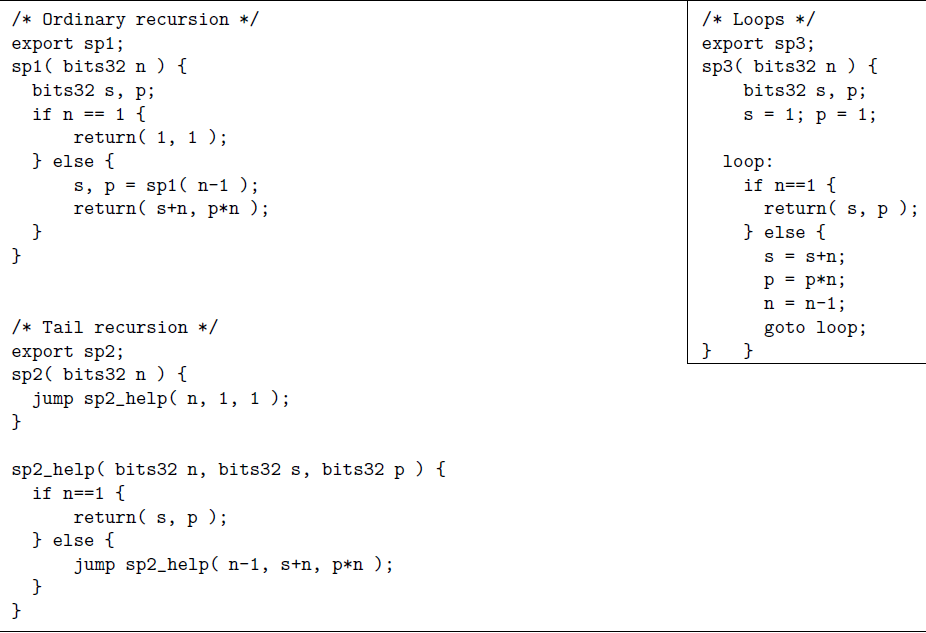
\includegraphics[scale=0.40]{resources/cmm.png}
	\end{center}
	\caption{Tri funkcije za izračunavanje sume i proizvoda prvih n brojeva u programskom jeziku C-\,-}
	\label{fig:cmm}
\end{figure}

Prikažimo rezultate korišćenja LLVM-a na jednostavnom primeru izračunavanja funkcije zadate na sledeći način:
\begin{itemize}
	\item ako je n parno, sledeći broj je n/2
	\item ako je n neparno, sledeći broj je 3*n+1
	\item ako je n jedan, stop
\end{itemize}

Cilj je da nađemo najdužu sekvencu za početne brojeve od jedan do milion. Sekvencu čini broj koraka dok ne stignemo do stopa. Kod napisan u Haskelu je:

\begin{verbatim}
import Data.Word

collatzLen :: Int -> Word32 -> Int
collatzLen c 1 = c
collatzLen c n | n `mod` 2 == 0 = collatzLen (c+1) $ n `div` 2
| otherwise      = collatzLen (c+1) $ 3*n+1

pmax x n = x `max` (collatzLen 1 n, n)

main = print . solve $ 1000000
where solve xs = foldl pmax (1,1) [2..xs-1]
\end{verbatim}

Kompilacijom ovog k\^{o}da različitim vrstama generisanja izvršnog k\^{o}da, dobijaju se vremena prikazana u tabeli \ref{tab:vremena}.

\begin{table}[h!]
	\begin{center}
		\caption{Različita vremena generisanja izvršnih k\^{o}dova}
		\begin{tabular}{||c|c|c|c||} \hline
			GHC-6.13 (NCG) & GHC-6.13 (C) & GHC-6.13 (LLVM) & GCC-4.4.3 \\ \hline
			2.876s & 0.576s & 0.516s & 0.335s \\ \hline
		\end{tabular}
		\label{tab:vremena}
	\end{center}
\end{table}


Iako se očekuje da NCG  ima najkraće vreme izvršavanja, jer se direktno prevodi na mašinski k\^{o}d, vidimo da u ovom jednostavnom primeru to nije slučaj.

Prethodni primer se može jednostavno paralelizovati. Odgovarajući Haskel k\^{o}d je:

\begin{verbatim}
import Control.Parallel
import Data.Word

collatzLen :: Int -> Word32 -> Int
collatzLen c 1 = c
collatzLen c n | n `mod` 2 == 0 = collatzLen (c+1) $ n `div` 2
| otherwise      = collatzLen (c+1) $ 3*n+1

pmax x n = x `max` (collatzLen 1 n, n)
main = print soln
where
solve xs = foldl pmax (1,1) xs
s1 = solve [2..500000]
s2 = solve [500001..999999]
soln = s2 `par` (s1 `pseq` max s1 s2)
\end{verbatim}

U programu je jednostavno ostvarena podela na dva dela i kombinovanje korišćenjem Haskelovih 'par' i 'pseq' funkcija, koje ukazuju kompajleru da paralelno realizuje dva dela s1 i s2. U ovom slučaju, vreme izvršavanja pomoću LLVM-a je:

GHC-6.13 (Parallel, LLVM): 0.312

%STG-mašina se koristi za mapiranje ne-striktnih funkcionalnih jezika u hardver računara. Razvijena je za potrebe GHC kompajlera, u kom se intenzivno koristi. Realizovana je kao interpreter, sa ciljem da bude jednostavna za analizu i korišćenje (eng. user-friendly). Neki autori smatraju STG-mašinu kao deo međujezika zajedno sa Core-om.
%Pun naziv STG-mašine (eng. Spineless Tagless Graph Reducing Machine) je nastao od pojmova G-mašina koja ima apstraktnu arhitekturu za obradu programa na funkcionalnom jeziku i pojmova: 
%spineless ukazuje da graf nije prikazan kao jedinstvena struktura podataka u memoriji, već kao skup manjih pojedinačnih delova grafa koji se međusobno referišu. Značajan deo mehanizma evaluacije čini deo koji se odnosi na referisanje tih delova.
%tagless ukazuje da su sve vrednosti na hipu (neizračunati izrazi, funkcije, već izračunati izrazi) prikazane na sličan način kroz zatvorenja (eng. closure). Ovo je obrnuto od tagfull, gde su zatvorenja anotirana podacima o tipu izraza i da li je izraz već izračunat.
%graph reducing ukazuje da izrazi na hipu mogu biti prepisani jednostavnijim vrednostima koje mašina smatra ekvivalentim početnom izrazu. Na primer, izračunavanje izraza 1+1 na hipu, može biti zamenjeno konstantom 2, pritom taj rezultat (2) je eventualno ostvaren na nekom drugom mestu.
%Ideja ove mašine je da predstavi program u formi apstraktnog sintaksnog drveta. Međutim, zbog referisanja delova sintaksnog drveta, program je u obliku grafa, a ne drveta. Evaluacijom tog grafa, korišćenjem malog broja instrukcija, sistematski ga redukujemo do krajnjeg oblika, što će biti rezultat izvršavanja programa.

%
%\begin{primer} Ovako se ubacuje slika. Obratiti pažnju da je dodato i 
%	\begin{verbatim}
%	\usepackage{graphicx}
%	\end{verbatim}
%	
%	\begin{figure}[h!]
%		\begin{center}
%			%\includegraphics[scale=0.75]{panda.jpg}
%		\end{center}
%		\caption{Pande}
%		\label{fig:pande}
%	\end{figure}
%	
%	Na svaku sliku neophodno je referisati se negde u tekstu. Na primer, na %slici \ref{fig:pande} prikazane su pande. 
%\end{primer}
%
%\begin{primer} I tabele treba da budu u svom okruženju, i na njih je neophodno referisati se u tekstu. Na primer, u tabeli% \ref{tab:tabela1} su prikazana različita poravnanja u tabelama.
%	
%	\begin{table}[h!]
%		\begin{center}
%			\caption{Razlčita poravnanja u okviru iste tabele ne treba koristiti jer su nepregledna.}
%			\begin{tabular}{|c|l|r|} \hline
%				centralno poravnanje& levo poravnanje& desno poravnanje\\ \hline
%				a &b&c\\ \hline
%				d &e&f\\ \hline
%			\end{tabular}
%			\label{tab:tabela1}
%		\end{center}
%	\end{table}
%	
%\end{primer}
\section{Zaključak}
\label{sec:zakljucak}

Implementacija funkcionalnih jezika predstavlja veoma težak posao i obimnu temu. U ovom radu fokus je na kompilaciji funkcionalnih jezika, najviše na procesu transformacije funkcionalnog koda u Haskel-u. Čitalac bi trebalo da, nakon čitanja ovog rada, bude upoznat sa teorijskim osnovama kompiliranja funkcionalnih jezika, razume transformaciju izvornog koda i bude u stanju da samostalno istražuje na ovu temu.
U našem radu smo se fokusirali na prevodenje izvnornog koda do mašinskog jezika. Taj proces se sastoji od 3 faze : frontend, middle end i backend. U radu su detaljno opisane kljucne faze za efikasnost prevodenja i jedan od najvažnijih razloga za, danas široku upotrebu Haskel jezika. Te faze su transformacija koda i LLVM framework.
GHC kompajler je u stalnom razvoju, a trenutno programeri se najviše fokusiraju na razvoj strategija izvođenja, razne strukture koje bi omogućile efikasniji rad skupljača djubreta(eng. \emph{garbage collector}) i na unapređenje izuzetaka pri prekorečenju heap memorije(dosadašnje verzije izbacuju nedostatke samo pri određenim okolnostima).



\addcontentsline{toc}{section}{Literatura}
\appendix
\bibliography{seminarski} 
\bibliographystyle{plain}

%\appendix
%\section{Dodatak}
Ovde pišem dodatne stvari, ukoliko za time ima potrebe.
Ovde pišem dodatne stvari, ukoliko za time ima potrebe.
Ovde pišem dodatne stvari, ukoliko za time ima potrebe.
Ovde pišem dodatne stvari, ukoliko za time ima potrebe.
Ovde pišem dodatne stvari, ukoliko za time ima potrebe.


\end{document}
